\documentclass[aspectratio=169, 10pt] {beamer}
\usetheme[faculty=phil]{fibeamer}
\usepackage[utf8]{inputenc}
\usepackage[main=english,]{babel}
\usepackage{subcaption}

\makeatletter
\renewcommand\fibeamer@includeLogo[2][]
\makeatother

\title{A Tool for Signal Chain Simulation in Particle Physics}
\subtitle{Octavio Gamez and Desiree Martinez} 
\author{July 31st, 2026}

\usepackage{ragged2e}  % `\justifying` text
\usepackage{booktabs}  % Tables
\usepackage{tabularx}
\usepackage{tikz}      % Diagrams
\usetikzlibrary{calc, shapes, backgrounds}
\usepackage{amsmath, amssymb}
\usepackage{url}       % `\url`s
\usepackage{listings}  % Code listings
\frenchspacing
\includegraphics[trim=left bottom right top, clip]{filename}

\begin{document}
\frame[c]{\maketitle}

%Slide 2
    \begin{frame}{Motivation}
    \large
    There are no widely known, open-source, tools that experimenters can use in order to plan their circuits without having a detailed schematic. \\

    %ADD PICTURE OF LIKE A PMT TO DIGITIZER TYPA TOOL IDK
    \end{frame}


%Slide 3
%     \begin{frame}{Gaps in Pre-Existing Tools}
%     SPICE simulators are accurate but not ideal or realistic during the early planning stages of an experiment\\

%     %ADD PICTURE OF A SPICE SIMULATOR 

%     \begin{figure}
%         \hfill
%         \includegraphics[width=0.7\linewidth]{SPICE.jpg}
%         \caption{Caption}
%         \label{fig  1:placeholder}
%     \end{figure}


%     \small
%     Figure 1: Electrical Engineering Oli Glaser
% %I cant figure out how to show this, i need the pic to be big but my text wont freaking go to the left side of the screen
    
%     %DURING PRESENTING WE CAN TALK ABOUT HOW IT IS ACCURACT BUT REQUIRES A FULLY DETAILED SCHEMATIC AND YEAH YA FEEL?
%     %MAYBE GO ONTO HOW THIS IS ONE OF THE OPTIONS BUT THE OTHER ONE IS TO JUST KEEP GOING WITH YOUR GUT AND  PAST EXPERIENCES WHICH ISNT IDEAL
%     \end{frame}


% %Slide 4
%     \begin{frame}{Project Goal}
%     \large
%     Design an open source tool for the pre-planning stage of an experiment that will report reflections, distortions, and signal loss

%     %IDK WHAT PICTURE YOUD WANT TO ADD
%     \end{frame}


    \begin{frame}{Project Goal}
        
        \centering
        {\Large Detector \to Analog \hspace{.4em} Electronics \to Digitizer \par} \\

        \vspace{1.5 cm}
         what reaches a computer is not always what left the detector 
    \end{frame}



    
    \begin{frame}{From a Particle Interaction to a Voltage Source}
        
        \centering
        {\Large Light \to Light \to Photoelectron \to Voltage \hspace{.4em} pulse \par} \\

        \vspace{1.5 cm}
         scintillator and photomultiplier tube  
    \end{frame}


%Slide 5 (MAYBE COULD ADD IDK IF IT WOULD BE RELEVENT BUT IT DONT MATTER
%    \begin{frame}{Understanding a signal}
%    Experimenters try to understand things they see in signals; 
%    \begin{itemize}
%        \item Source
%        \item Timing
%        \item Reflections
%        \item Distortions
%        \item Signal Loss
%    \end{itemize}

    %ADD PIC OF SIGNAL AND POINT OUT THE PARTS OF THE SIGNAL IDK
%    \end{frame}
%GET RID OF THE PERCENTAGE SIGNS IF YOU WANT TO ADD IT

\begin{frame}{Reflections}
    Reflection Coefficient:
$$\Gamma = \frac{(Z_{\text{load}} - Z_0)}{(Z_{\text{load}} + Z_0)}$$
 \vspace{2}
 \setlength{\fboxsep}{10pt}
 \centering\fbox{Z_S} ------------------------------------------------\fbox{Z_L}\\
 \uparrow \\
 Z_0
 
\end{frame}


\begin{frame}{Simulation Structure}
 \setlength{\fboxsep}{10pt}
 \centering\fbox{  PMT  } \fbox{  Cable   } \fbox{   Splitter  } \fbox{  Discriminator  } \fbox{Amplifier} \fbox{Digitizer} \\

 \vspace{1.5cm}

 Component level simulation
 
\end{frame}




\begin{frame}{Design: Normalize the Bi-Exponential}
    \begin{columns}[c] % [c] centers the content vertically
        
        % Left Column: Math Formulas & Notes
        \begin{column}{0.5\textwidth}
            $$
            f(t) =  \frac{e^{-\frac{t}{\tau_{\text{fall}}}} - e^{-\frac{t}{\tau_{\text{rise}}}}}
            {\tau_{\text{fall}} - \tau_{\text{rise}}}  
            $$
            
            $$
            \int_{0}^{\infty} f(t) \, dt = 1 
            $$
            

        \end{column}
        
        % Right Column: Image
        \begin{column}{0.9\textwidth}
            \centering
            \hspace{-3.5cm}
            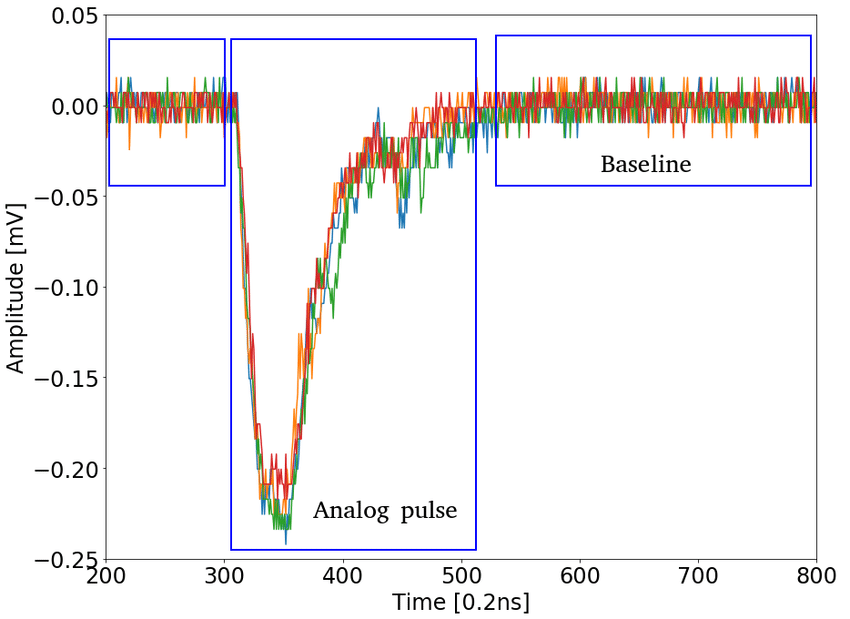
\includegraphics[ width= 0.7\linewidth]{PMTPULSE.png}
        \end{column}
        
    \end{columns}
\end{frame}



\begin{frame}{Design: Generate individual photoelectrons}
\centering
\lambda(t)  = N*f(t)

Poisson Arrivals \to Single \hspace{.4em} photoelectron \hspace{.4em} pulses \to Sum \hspace{.4em} single photoelectron\hspace{.8em}  pulses

\end{frame}



\begin{frame}{Design: Voltage Convention}
    \begin{columns}[c] % [c] vertically centers the content in both columns
        
        \begin{column}{0.45\linewidth}
            \raggedright % 
            Output waveform and output impedance 
        \end{column}
        
       
        \begin{column}{0.5\linewidth}
            \centering
            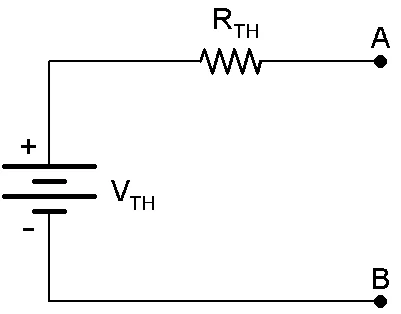
\includegraphics[width=\linewidth]{thenevin.png}
        \end{column}
        
    \end{columns}
\end{frame}

%Slide 7



\begin{frame}{PMT}
    PMT &\quad\\  

    \begin{figure}
        \centering
        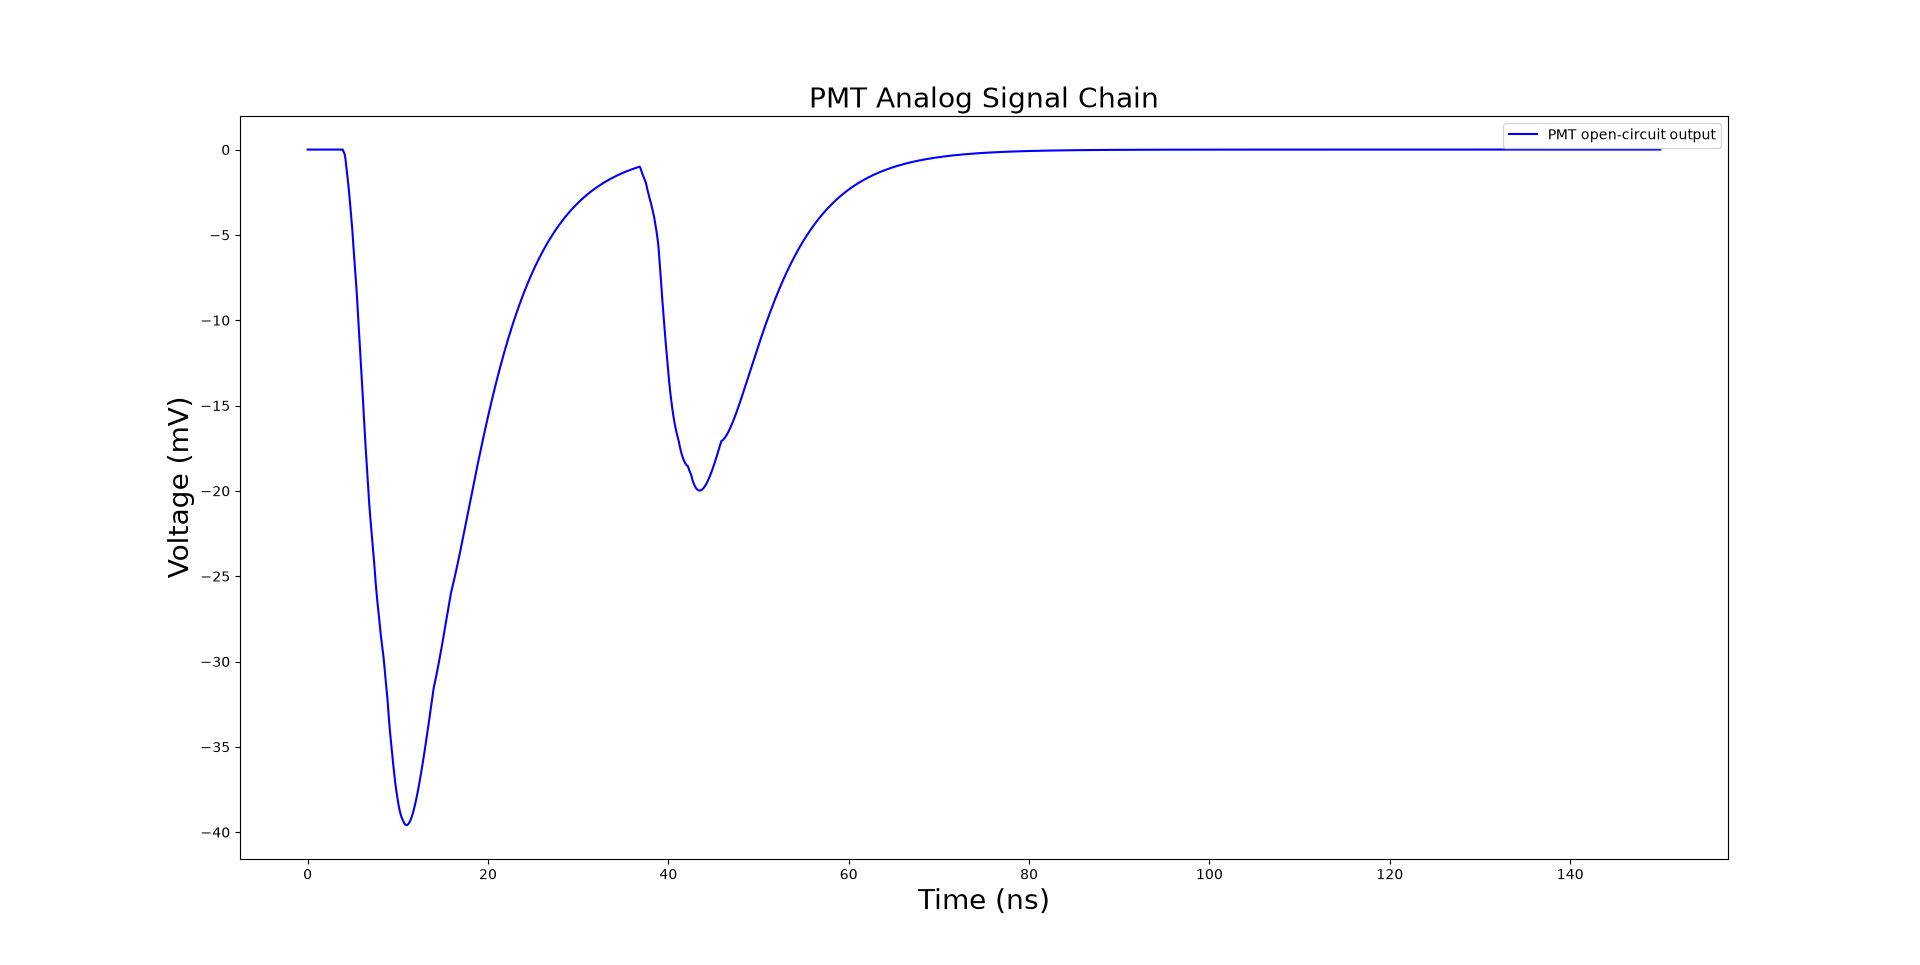
\includegraphics[trim=3cm 2cm 1.9cm 3cm, clip, width=1.0\linewidth]{PMTSignal.png} 
        \caption{Synthetic PMT Pulse}
        \label{fig:placeholder}
    \end{figure}
    
\end{frame}




\begin{frame}{Cable}
    PMT \to \text{1m 50 $\Omega$ cable} \\
     \begin{figure}
        \centering
        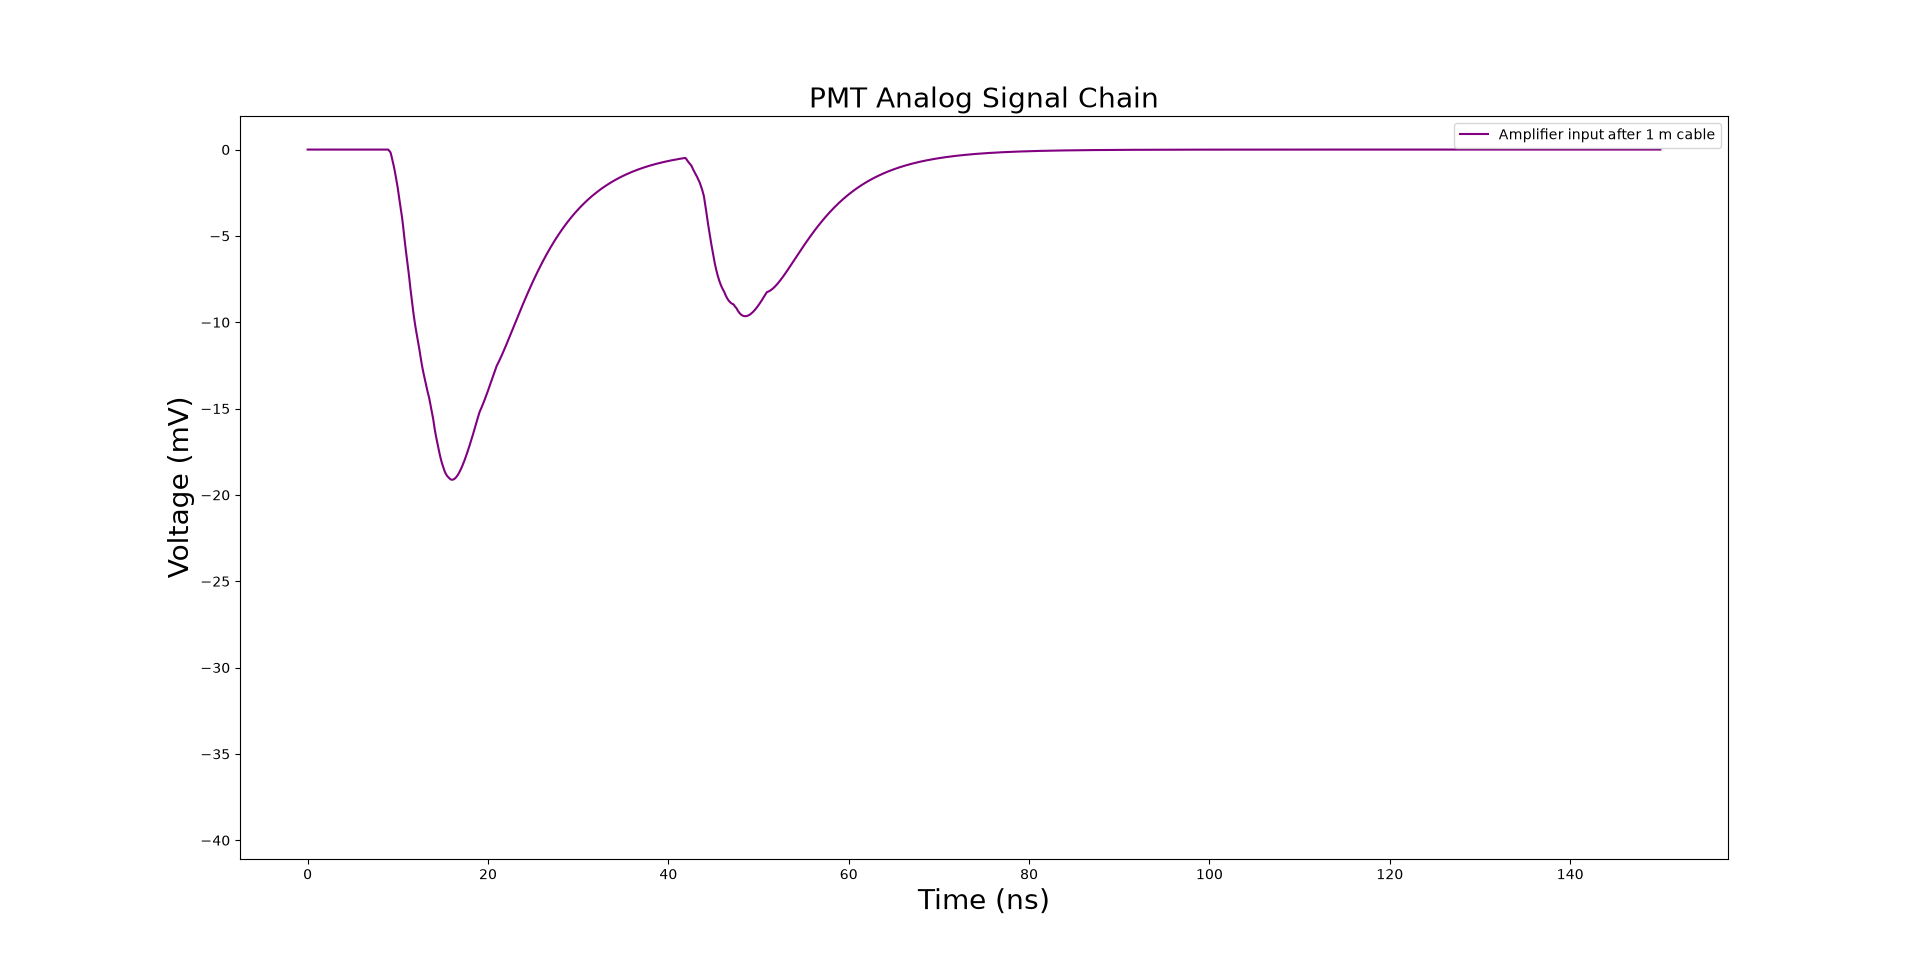
\includegraphics[trim=3cm 2cm 1.9cm 3cm, clip, width=1.0\linewidth]{AMP_IN.png} 
        \caption{pulse after being ran through the cable}
        \label{fig:placeholder}
    \end{figure}
\end{frame}


\begin{frame}{Amplifier}
    PMT \to \text{1m 50 $\Omega$ cable} \to Amplifier \\
     \begin{figure}
        \centering
        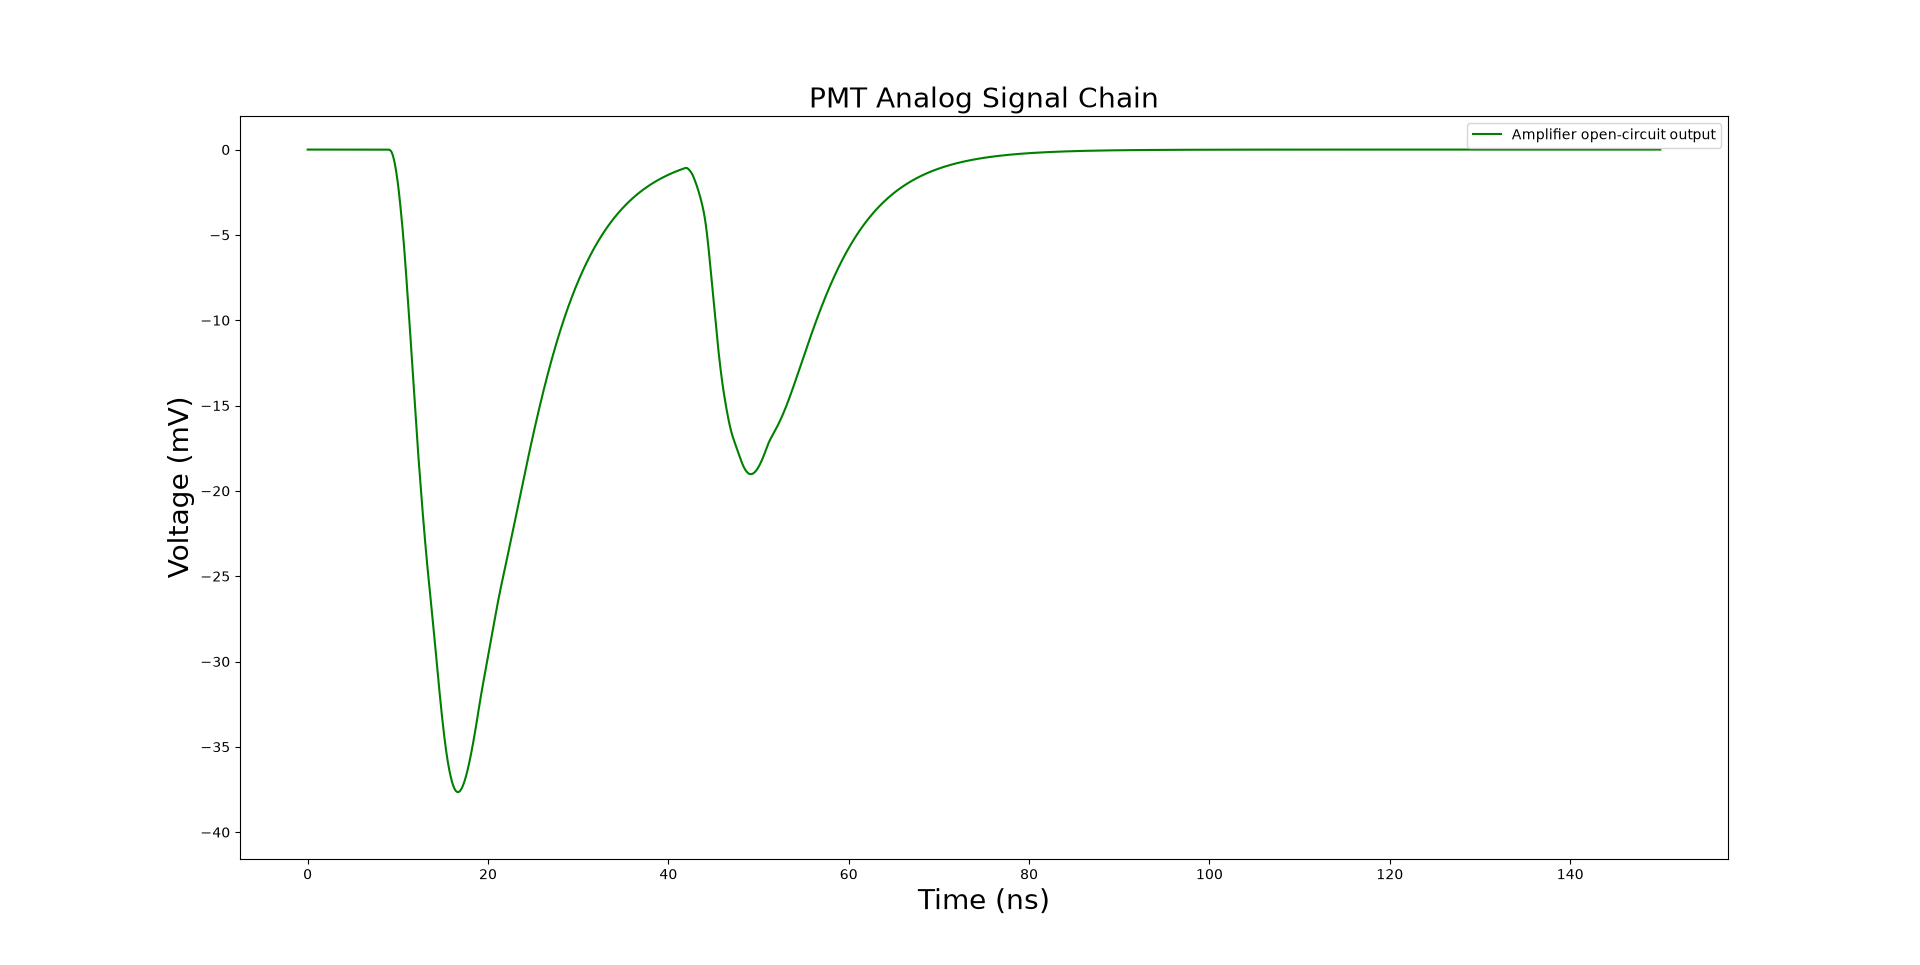
\includegraphics[trim=3cm 2cm 1.9cm 3cm, clip, width=1.0\linewidth]{AMP_OPEN_CIRCUIT.png} 
        \caption{Pulse After Being Ran Rhrough Amplifier}
        \label{fig:placeholder}
    \end{figure}
\end{frame}


\begin{frame}{Cable}
    PMT \to \text{50 $\Omega$ cable} \to Amplifier \to \text{5m 100 $\Omega$ cable} \\
     \begin{figure}
        \centering
        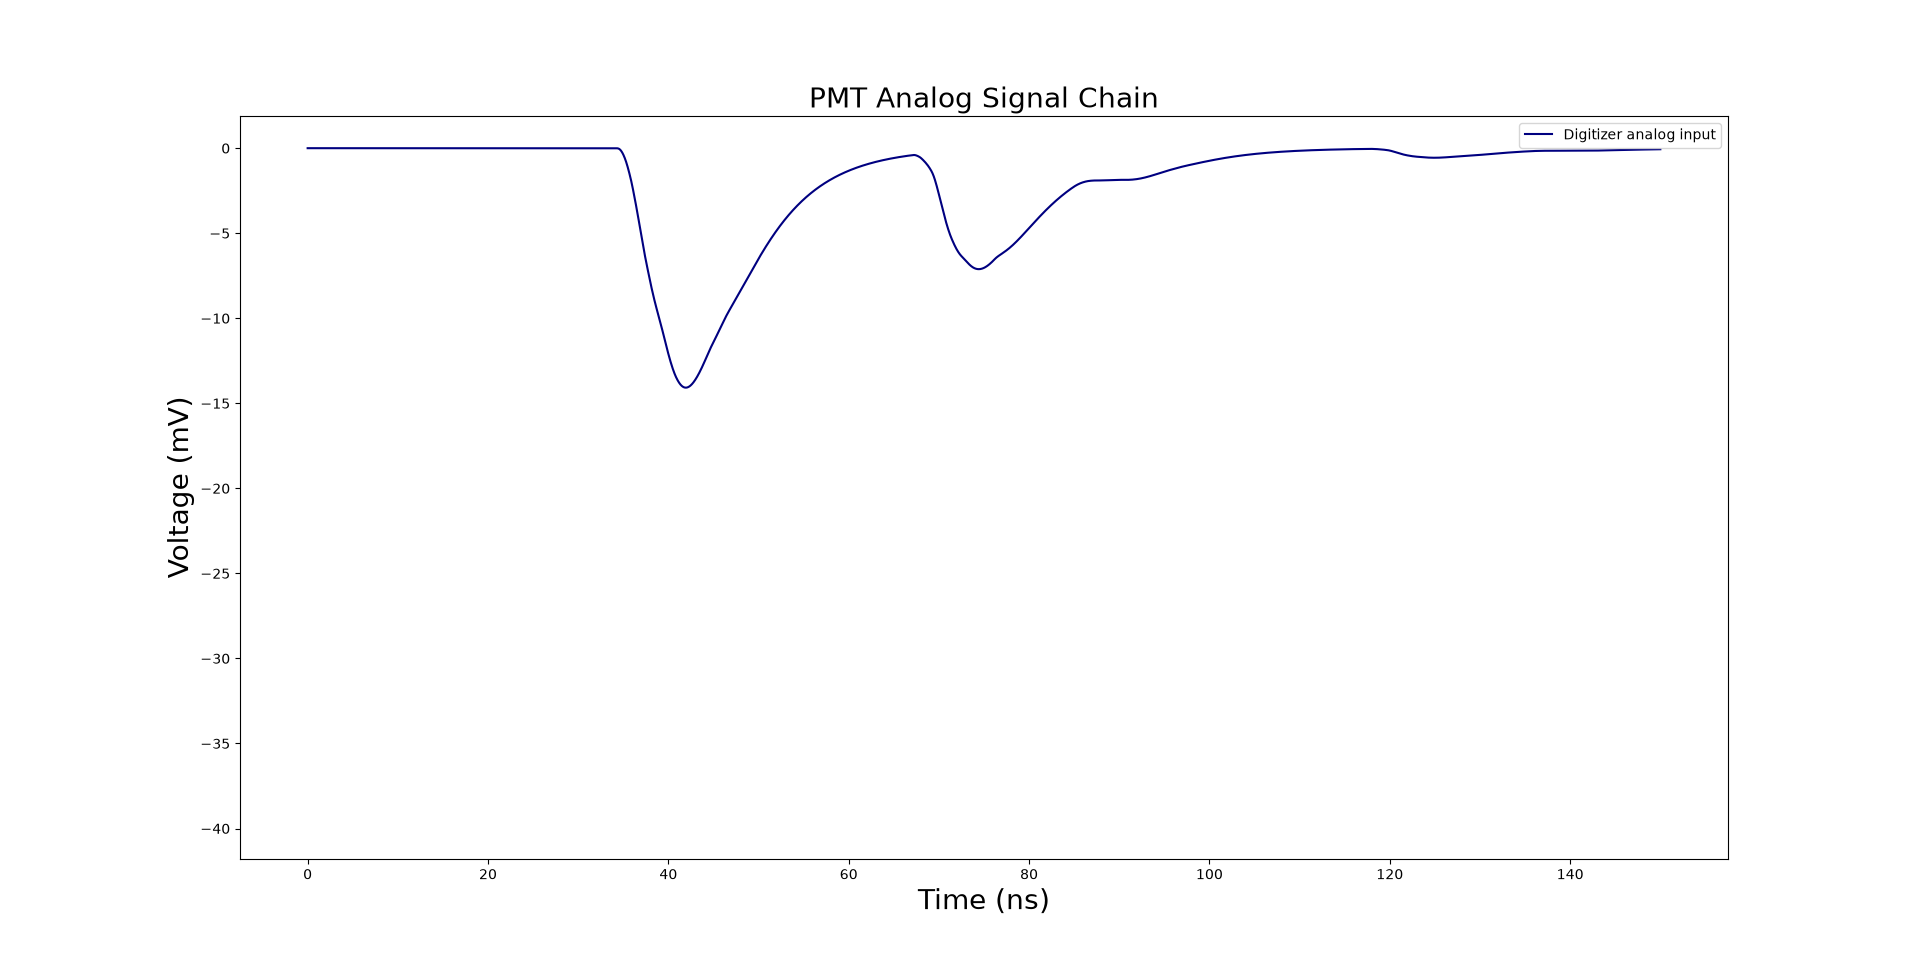
\includegraphics[trim=3cm 2cm 1.9cm 3cm, clip, width=1.0\linewidth]{DIG_ANALOG_INPUT.png} 
        \caption{Synthetic PMT Pulse}
        \label{fig:placeholder}
    \end{figure}
\end{frame}


\begin{frame}{Digitizer}
    PMT \to \text{50 $\Omega$ cable} \to Amplifier \to \text{5m 100 $\Omega$ cable} \to Digitizer \\
     \begin{figure}
        \centering
        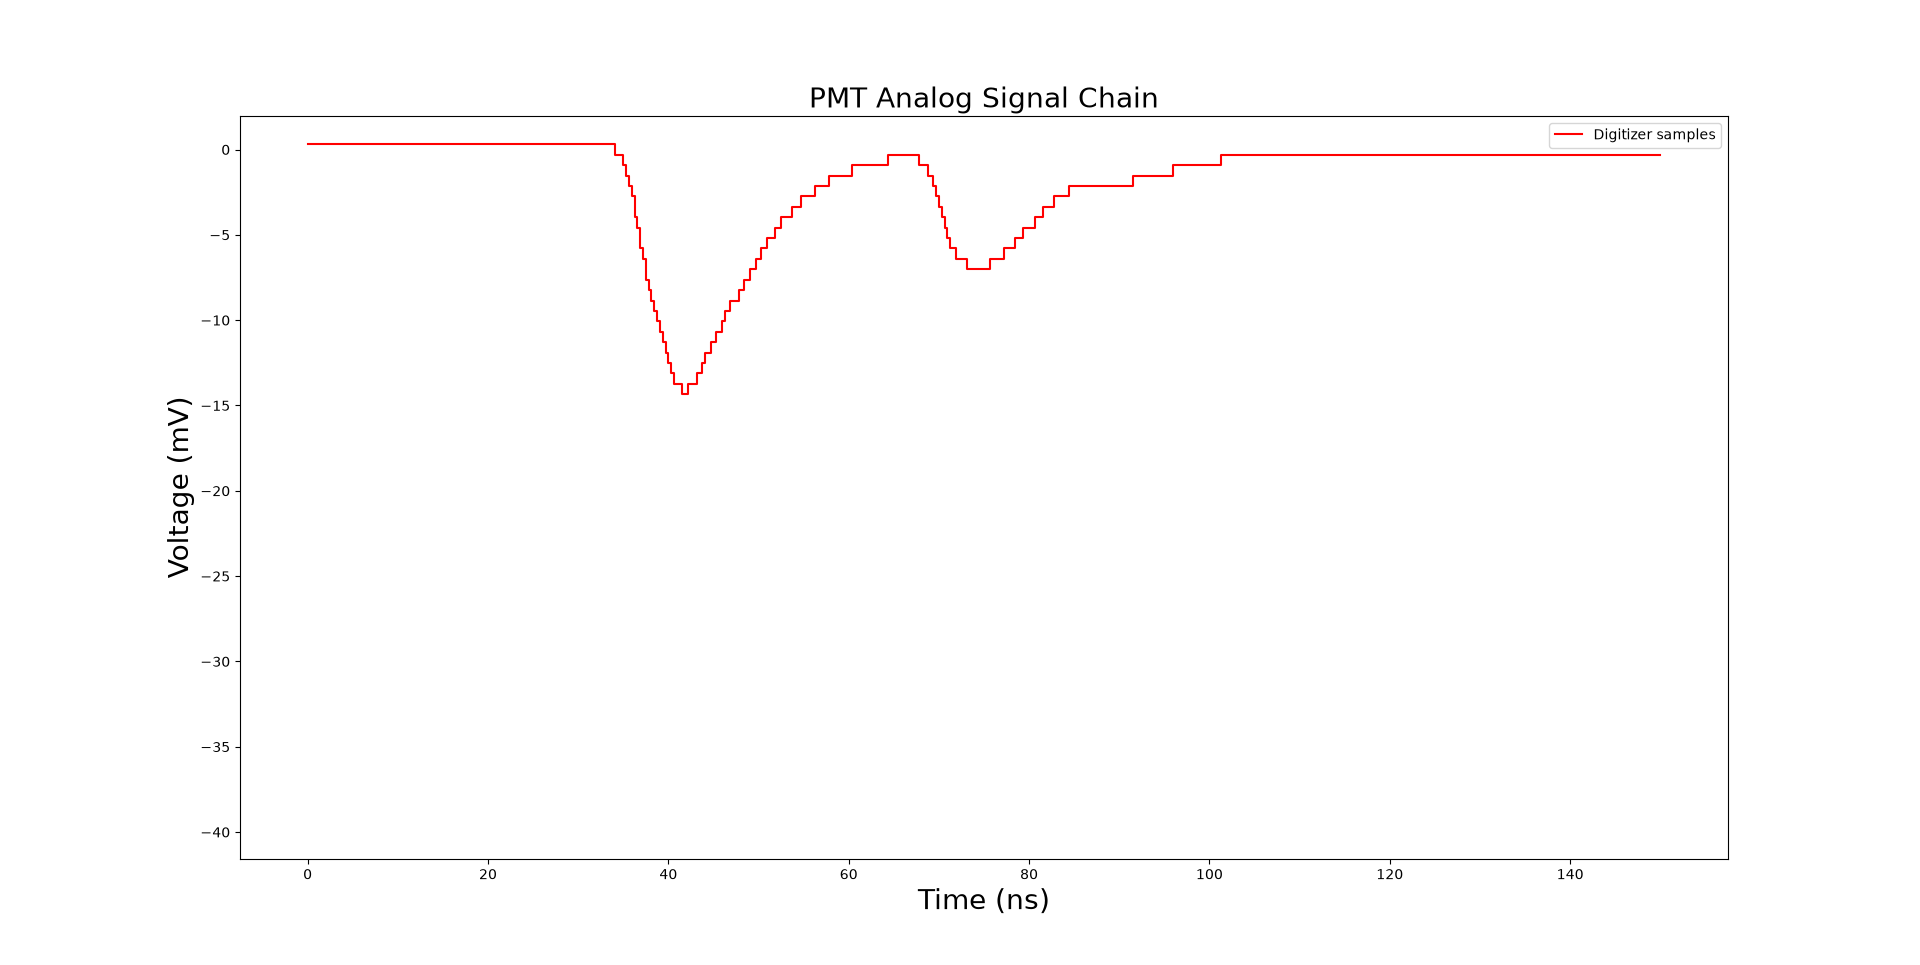
\includegraphics[trim=3cm 2cm 1.9cm 3cm, clip, width=1.0\linewidth]{DIGITIZED.png} 
        \caption{Digitized signal}
        \label{fig:placeholder}
    \end{figure}
\end{frame}


\begin{frame}{Digitizer}
    PMT \to \text{50 $\Omega$ cable} \to Amplifier \to \text{5m 100 $\Omega$ cable} \to Digitizer \\
     \begin{figure}
        \centering
        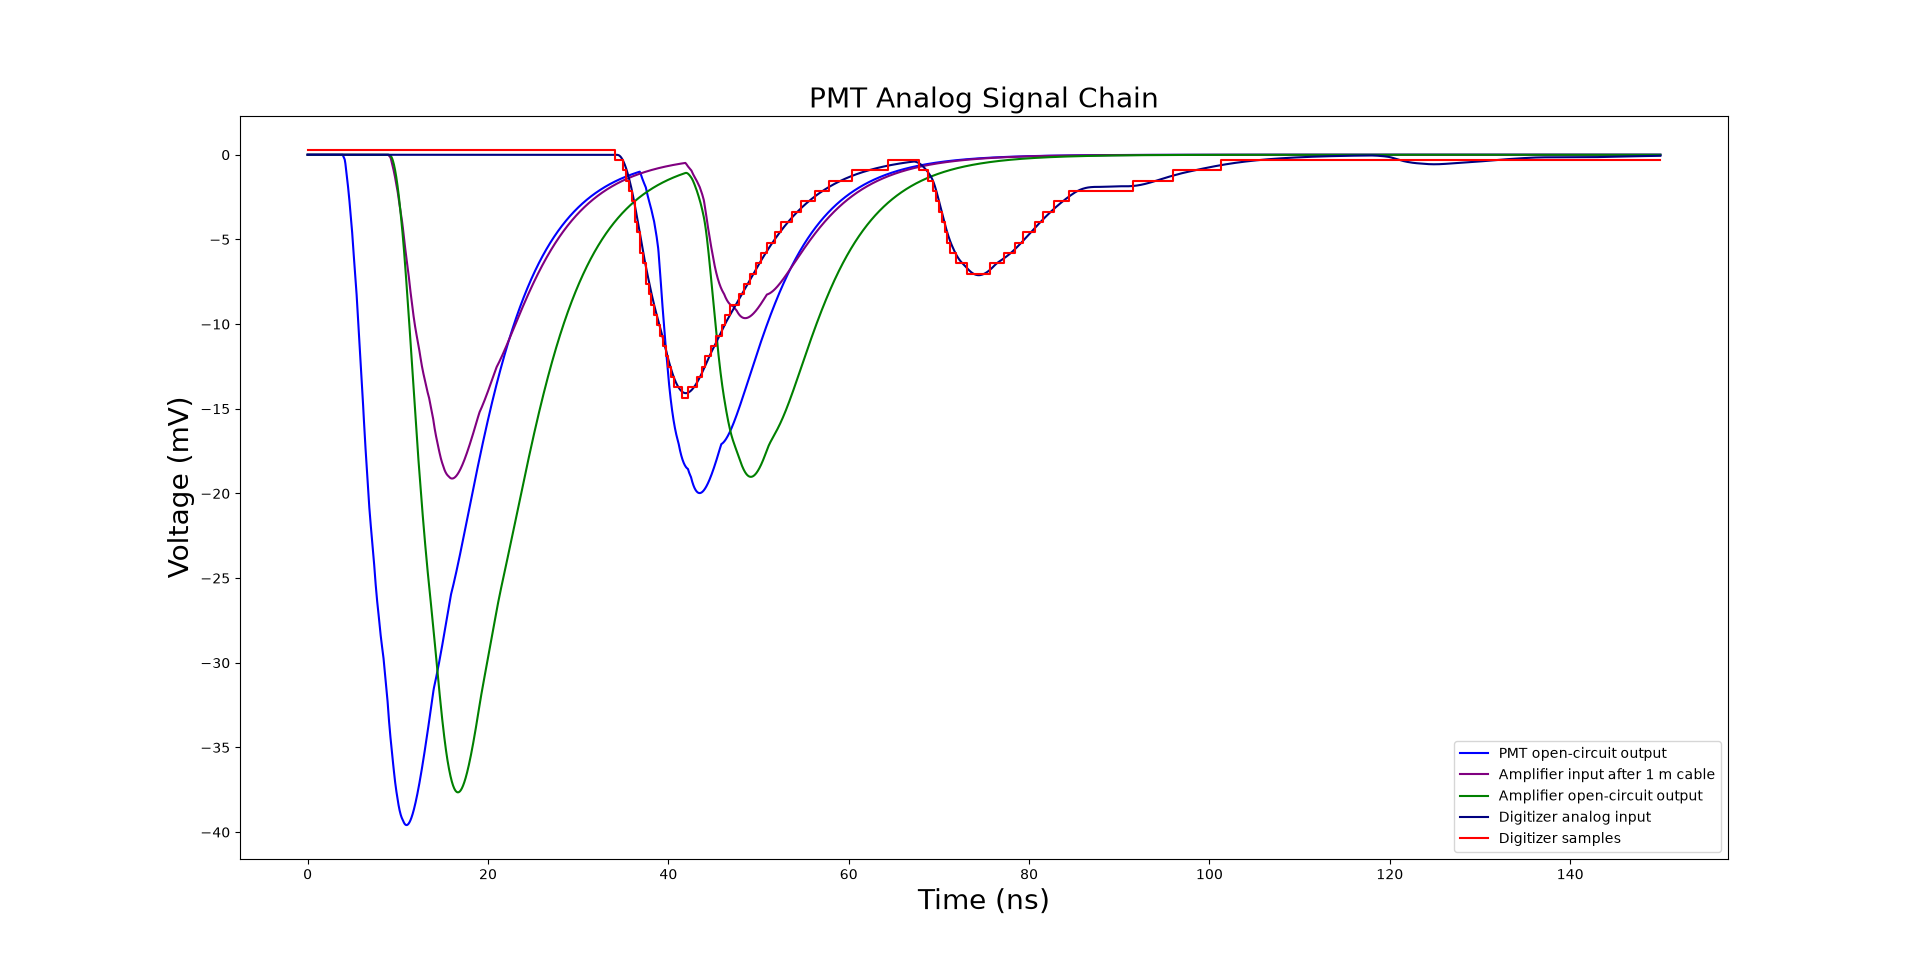
\includegraphics[trim=3cm 2cm 1.9cm 3cm, clip, width=1.0\linewidth]{ALLTOGETHER.png} 
        \caption{Journey of the pulse}
        \label{fig:placeholder}
    \end{figure}
\end{frame}


\begin{frame}{Next Steps}
\begin{itemize}
    \item Compare simulated pulses to measured ones 
    \item Expand detector support 
    \item Enhancing different features that are already implemented in our design
\end{itemize}
    
\end{frame}

\end{document}
